\message{ !name(neuralfields.tex)}%%
%% neuralfields.tex
%% 
%% Made by jjfigueredou
%% Login   <jjfigueredou@fctp-jjfu>
%% 
%% Started on  Sun Oct  5 12:26:22 2008 jjfigueredou
%% Last update Sun Oct  5 12:26:22 2008 jjfigueredou
%%
\documentclass[preprint]{sigplanconf}
\usepackage[latin1]{inputenc}
\usepackage[numbers]{natbib}
\usepackage[english]{babel}
\usepackage{graphicx}
\usepackage{algorithm}
\usepackage{algorithmic}
\usepackage{amsmath}

\begin{document}

\message{ !name(neuralfields.tex) !offset(178) }
\subsection{Recurrent neural control architecture}
The proposed architecture for the recurrent neural network controller
has two expert recurrent networks, whose interaction will achieve
positioning and equilibrium as well.

There has been applied a preprocessing stage previous to the input
neurons, so that the actual values are not used and instead the inputs
are mapped to 3 fuzzy sets. In this way, the stability controller only
has 3 inputs, while the positioning controller has 6, corresponding to
the same 3 inputs previously described and another 3 due to the fuzzy
mapping of the error signal. All neurons are interconnected and the
first one of them is selected as output without loss of
generality. The neural network topology for the first controller
(stability) is shown in the figure 1.

\begin{figure}[t]
\centering
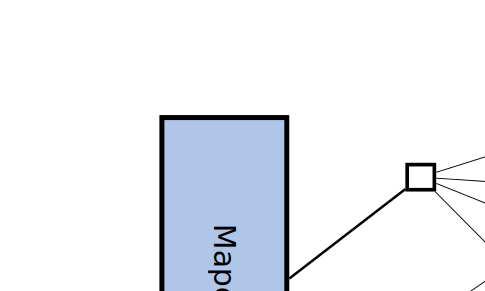
\includegraphics[width=7cm]{rnn.png}
\caption{Neural net for stability control including fuzzy mapping}
\label{rnn}
\end{figure}

\message{ !name(neuralfields.tex) !offset(322) }

\end{document}